\chapter{A convolutional neural network for CHIPS}
\label{chap:cvn}

\begin{comment}
STORY OF THE CHAPTER

There are many standard ways that event classification and paramter (mainly energy) estimation are
usually done in HEP. These mainly include the reconstruction of objects and their associated parameters
wether these are clusters, tracks, jets or cherenkov rings. Typically these along with other constructed
features are then passed through a simple machine learning model for event or particle classification, or
combined in some other way for energy estimation.

While this has worked leveraging the enormous amount of work in machine learning especially deep learning
surely would prove valuable. The key thing that has been done is to move away from human engineered features
to machine learning models that discover the underlying features that work best in clasifiying of regressing
a particualar task.

Water chernkov detectors are especially paired to this task as the output from our detectors is essentially
an 'image' of the event and so classification models that work well on images shoud work well on
seperating our types of events.

Firstly, the principle issue with matching water cherenkov detectors and deep learning is representing the cylindrical
detector output of either a 2d flat map that a typically conv network can use as input of use a more complicated
graph network approach as some other people have tried. Typically people have just ignored the endcaps, but
this is not optimal as these contain nearing half the detected light in a standard CHIPS detector. Other appraoches
include the x+ x- approach. But as hited at by tomothy report, for a primarilly event classification task,
removing any distritions due to the detector shape is the most important things. Therefore, the approach of
veiwing the "image" from the interaction vertex point preserves the cherenkov ring strucutre as best possible.

The hough space is used to find this vertex and direction from which the images are produces, so it also made sense
to include this along with time as a seperate channel in the output. You can see fro the vertext position is best. Using
a more unformly distributes sample of events leads to a greater abiity to distinguish the types which is important
for subsequant energy reconstruction.

Many possible models have been developed for convolutional neural networks over th years.

Firstly, the principle issue with matching water cherenkov detectors and deep learning is representing the cylindrical
detector output of either a 2d flat map that a typically conv network can use as input of use a more complicated
graph network approach as some other people have tried. Typically people have just ignored the endcaps, but
this is not optimal as these contain nearing half the detected light in a standard CHIPS detector. Other appraoches
include the x+ x- approach. But as hited at by tomothy report, for a primarilly event classification task,
removing any distritions due to the detector shape is the most important things. Therefore, the approach of
veiwing the "image" from the interaction vertex point preserves the cherenkov ring strucutre as best possible.

Introduction (tell them what you are going to tell them)
- Previous applications in HEP

Theory (tell them what they need to know to understand)
- How basic neural networks work
- How convolutional neural networks build ontop of this
- The problem of overfitting


- Previous applications in HEP
- A baseline implementation for CHIPS
- Conclusion (tell them what you told them)

TODO: Read through all CVN related papers and make general notes in appropriate subsections
\end{comment}

%%%%%%%%%%%%%%%%%%%%%%%%%%%%%%%%%%%%%%%%%%%%%%%%%%%%%%%%%%%%%%%%%%%%%%%%%%%%%%%%%%%%%%%%%%%%%%%%%%%%%%%%%%%%%%%%%%
%                                                 INTRODUCTION                                                   %
%%%%%%%%%%%%%%%%%%%%%%%%%%%%%%%%%%%%%%%%%%%%%%%%%%%%%%%%%%%%%%%%%%%%%%%%%%%%%%%%%%%%%%%%%%%%%%%%%%%%%%%%%%%%%%%%%%
\section{Introduction}
\label{sec:cvn_intro}
- Standard water cherenkov analysis is via a likelihood hood fit to the ring assuming some event topology hypothesis.
- This is used in super-k with fitqun and what has been previously implemented for CHIPS in the WCSimAnalysis package.
- Previous work in HEP has applied deep learning to a variety of problems...

%%%%%%%%%%%%%%%%%%%%%%%%%%%%%%%%%%%%%%%%%%%%%%%%%%%%%%%%%%%%%%%%%%%%%%%%%%%%%%%%%%%%%%%%%%%%%%%%%%%%%%%%%%%%%%%%%%
%                                                    Theory                                                      %
%%%%%%%%%%%%%%%%%%%%%%%%%%%%%%%%%%%%%%%%%%%%%%%%%%%%%%%%%%%%%%%%%%%%%%%%%%%%%%%%%%%%%%%%%%%%%%%%%%%%%%%%%%%%%%%%%%
\section{Theory}
\label{sec:cvn_theory}
- Take insights from neuroscience. The human eye can do remarkably well at image recognition, even neutrino event classification if
you know what to look for. But we will have way too much data, so need to train a computer to do this task for us.
- A MPL with a single hidden layer can be shown to apprximate any function arbitrarily accurately. Give REF for this.
- Conv is a set of 'filters' that when applied via scanning across an input image result in a feature map
- Pooling used as each layer requires less complexity and it is less important about the location and that the feature exists.
- Few learners search their hypothesis space fully. Therefore, a learner with a large hypothesis space that tries fewer hypotheses from it is less likely to overfit than one that tries more hypotheses from a smaller space.
- All that "deep" really means is just many many hidden layers, which can encode complex structures more efficienctly.
- They can be very difficult to train, but with GPUs, bigger training sets, weight inits, better non linearities, SGD, prevention of overfitting techniques and conv networks, its possible.

\begin{equation} % NETWORK BASIC EQUATION %%%%%%%%%%%%%%%%%%%%%%%%%%%%%%%%%%%
    z^{(i)}=\boldsymbol{w}^{(i)}\cdot\boldsymbol{x}+b^{(i)}
\end{equation} %%%%%%%%%%%%%%%%%%%%%%%%%%%%%%%%%%%%%%%%%%%%%%%%%%%%%%%%%%%%%%

\begin{equation} % NETWORK ACTIVATION EQUATION %%%%%%%%%%%%%%%%%%%%%%%%%%%%%%
    a_{i}(\boldsymbol{x})=\sigma_i(z^{(i)})
\end{equation} %%%%%%%%%%%%%%%%%%%%%%%%%%%%%%%%%%%%%%%%%%%%%%%%%%%%%%%%%%%%%%

\begin{equation} % MEAN-SQUARED ERROR LOSS EQUATION %%%%%%%%%%%%%%%%%%%%%%%%%
    E(\boldsymbol{w})=
    \frac{1}{n}\displaystyle\sum_{i=1}^{n}(y_{i}-
    \hat{y}_{i}(\boldsymbol{w}))^{2}
\end{equation} %%%%%%%%%%%%%%%%%%%%%%%%%%%%%%%%%%%%%%%%%%%%%%%%%%%%%%%%%%%%%%

\begin{equation} % BINARY CROSS-ENTROPY EQUATION %%%%%%%%%%%%%%%%%%%%%%%%%%%%
    E(\boldsymbol{w})=
    -\displaystyle\sum_{i=1}^{n}y_{i}\log\hat{y}_{i}(\boldsymbol{w})+
    (1-y_{i})\log[1-\hat{y}_{i}(\boldsymbol{w})]
\end{equation} %%%%%%%%%%%%%%%%%%%%%%%%%%%%%%%%%%%%%%%%%%%%%%%%%%%%%%%%%%%%%%

\begin{equation} % CATEGORICAL CROSS-ENTROPY EQUATION %%%%%%%%%%%%%%%%%%%%%%%
    E(\boldsymbol{w})=
    -\displaystyle\sum_{i=1}^{n}\displaystyle\sum_{m=0}^{M-1}y_{im}\log\hat{y}_{im}(\boldsymbol{w})+
    (1-y_{im})\log[1-\hat{y}_{im}(\boldsymbol{w})]
\end{equation} %%%%%%%%%%%%%%%%%%%%%%%%%%%%%%%%%%%%%%%%%%%%%%%%%%%%%%%%%%%%%%

EQUATION: Batch-normalisation equations
EQUATION: Back propogation equations derivation and explanation

\begin{figure} % BASIC NETWORK DIAGRAM %%%%%%%%%%%%%%%%%%%%%%%%%%%%%%%%%%%%%%
    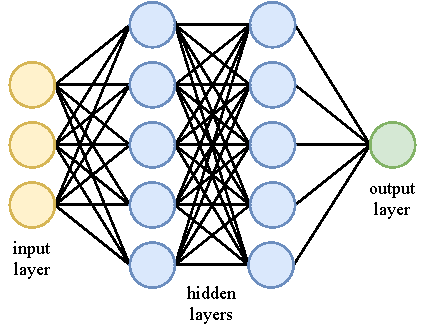
\includegraphics[width=0.8\textwidth]{diagrams/6-cvn/network.pdf}
    \caption[network short]
    {network long}
    \label{fig:network}
\end{figure} %%%%%%%%%%%%%%%%%%%%%%%%%%%%%%%%%%%%%%%%%%%%%%%%%%%%%%%%%%%%%%%%

\begin{figure} % DROPOUT DIAGRAM %%%%%%%%%%%%%%%%%%%%%%%%%%%%%%%%%%%%%%%%%%%%
    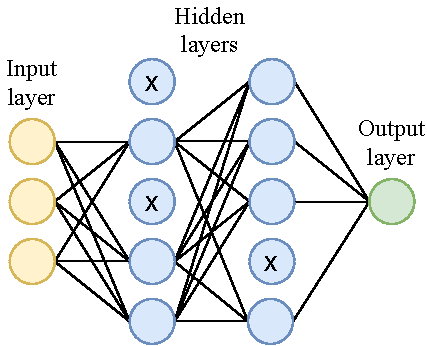
\includegraphics[width=0.8\textwidth]{diagrams/6-cvn/dropout.pdf}
    \caption[dropout short]
    {dropout long}
    \label{fig:dropout}
\end{figure} %%%%%%%%%%%%%%%%%%%%%%%%%%%%%%%%%%%%%%%%%%%%%%%%%%%%%%%%%%%%%%%%

\begin{figure} % ACTIVATIONS DIAGRAM %%%%%%%%%%%%%%%%%%%%%%%%%%%%%%%%%%%%%%%%
    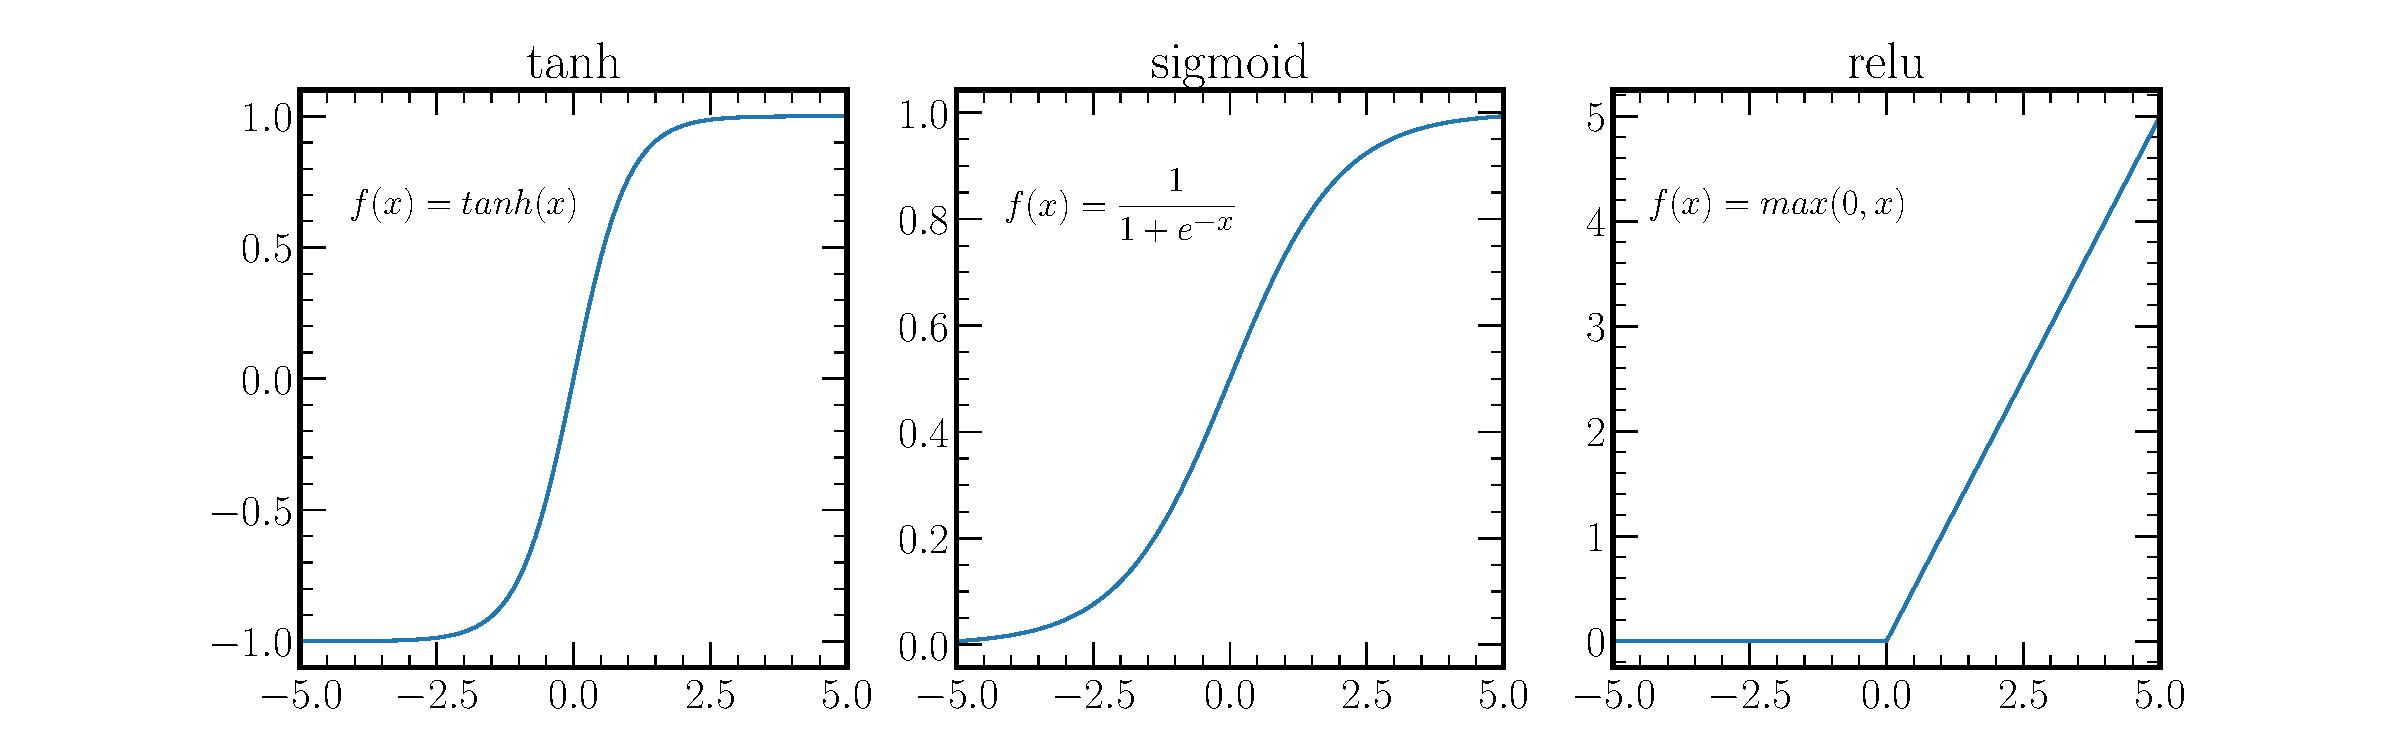
\includegraphics[width=\textwidth]{diagrams/6-cvn/activations.pdf}
    \caption[activations short]
    {activations long}
    \label{fig:activations}
\end{figure} %%%%%%%%%%%%%%%%%%%%%%%%%%%%%%%%%%%%%%%%%%%%%%%%%%%%%%%%%%%%%%%%

\begin{figure} % GRADIENT DESCENT DIAGRAM %%%%%%%%%%%%%%%%%%%%%%%%%%%%%%%%%%%
    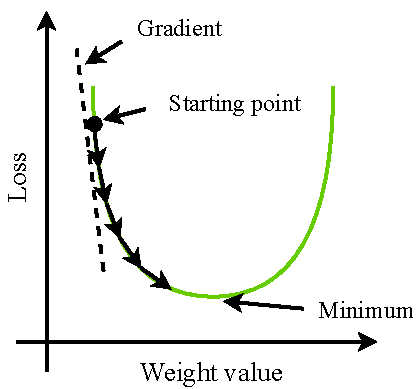
\includegraphics[width=0.8\textwidth]{diagrams/6-cvn/gradient_descent.pdf}
    \caption[gradient descent short]
    {gradient descent long}
    \label{fig:gradient_descent}
\end{figure} %%%%%%%%%%%%%%%%%%%%%%%%%%%%%%%%%%%%%%%%%%%%%%%%%%%%%%%%%%%%%%%%

\begin{figure} % CONV INPUTS DIAGRAM %%%%%%%%%%%%%%%%%%%%%%%%%%%%%%%%%%%%%%%%
    \centering
    \begin{subfigure}[b]{0.4\textwidth}
        \centering
        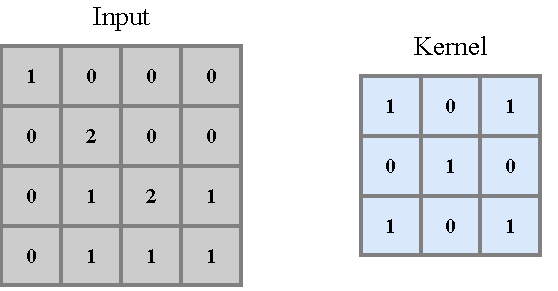
\includegraphics[width=\textwidth]{diagrams/6-cvn/conv_input.pdf}
        \caption{conv input long}
        \label{fig:conv_input}
    \end{subfigure}
    \hfill
    \begin{subfigure}[b]{0.4\textwidth}
        \centering
        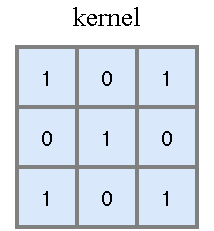
\includegraphics[width=\textwidth]{diagrams/6-cvn/conv_kernel.pdf}
        \caption{conv kernel long}
        \label{fig:conv_kernel}
    \end{subfigure}
    \caption{conv input and kernel}
    \label{fig:conv_input_kernel}
\end{figure} %%%%%%%%%%%%%%%%%%%%%%%%%%%%%%%%%%%%%%%%%%%%%%%%%%%%%%%%%%%%%%%%

TODO: combine the same and valid conv operations into the same diagram
\begin{figure} % CONV OPERATION DIAGRAM %%%%%%%%%%%%%%%%%%%%%%%%%%%%%%%%%%%%%
    \centering
    \begin{subfigure}[b]{0.71\textwidth}
        \centering
        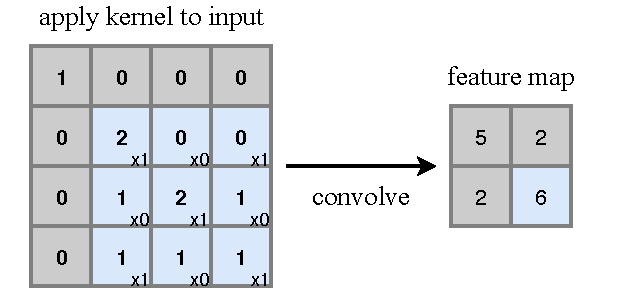
\includegraphics[width=\textwidth]{diagrams/6-cvn/conv_valid.pdf}
        \caption{conv valid long}
        \label{fig:conv_valid}
    \end{subfigure}
    \hfill
    \begin{subfigure}[b]{0.9\textwidth}
        \centering
        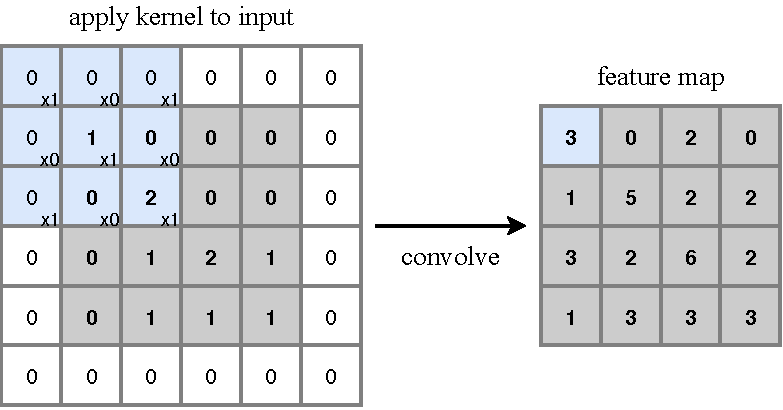
\includegraphics[width=\textwidth]{diagrams/6-cvn/conv_same.pdf}
        \caption{conv same long}
        \label{fig:conv_same}
    \end{subfigure}
    \caption{conv operations}
    \label{fig:conv_operations}
\end{figure} %%%%%%%%%%%%%%%%%%%%%%%%%%%%%%%%%%%%%%%%%%%%%%%%%%%%%%%%%%%%%%%%


\begin{figure} % POOLING DIAGRAM %%%%%%%%%%%%%%%%%%%%%%%%%%%%%%%%%%%%%%%%%%%%
    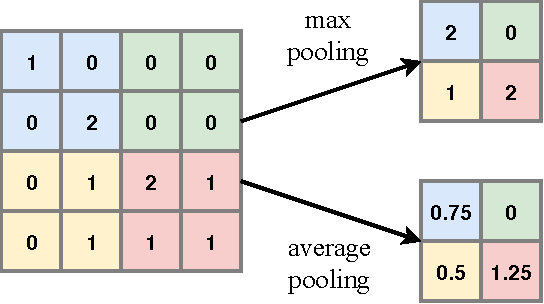
\includegraphics[width=0.8\textwidth]{diagrams/6-cvn/pooling.pdf}
    \caption[pooling short]
    {pooling long}
    \label{fig:pooling}
\end{figure} %%%%%%%%%%%%%%%%%%%%%%%%%%%%%%%%%%%%%%%%%%%%%%%%%%%%%%%%%%%%%%%%


\begin{figure} % EARLY STOPPING DIAGRAM %%%%%%%%%%%%%%%%%%%%%%%%%%%%%%%%%%%%%
    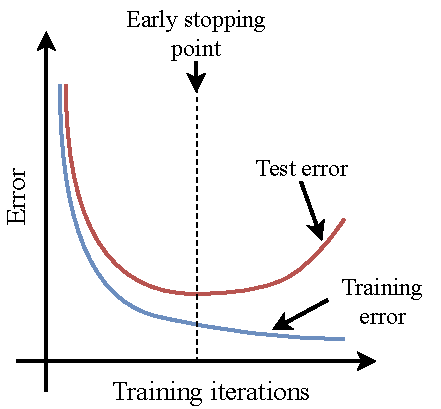
\includegraphics[width=0.8\textwidth]{diagrams/6-cvn/early_stopping.pdf}
    \caption[early stopping short]
    {early stopping long}
    \label{fig:early_stopping}
\end{figure} %%%%%%%%%%%%%%%%%%%%%%%%%%%%%%%%%%%%%%%%%%%%%%%%%%%%%%%%%%%%%%%%


%%%%%%%%%%%%%%%%%%%%%%%%%%%%%%%%%%%%%%%%%%%%%%%%%%%%%%%%%%%%%%%%%%%%%%%%%%%%%%%%%%%%%%%%%%%%%%%%%%%%%%%%%%%%%%%%%%
%                                                A CNN FOR CHIPS                                                 %
%%%%%%%%%%%%%%%%%%%%%%%%%%%%%%%%%%%%%%%%%%%%%%%%%%%%%%%%%%%%%%%%%%%%%%%%%%%%%%%%%%%%%%%%%%%%%%%%%%%%%%%%%%%%%%%%%%
\section{A CNN for CHIPS}
\label{sec:cvn_cnn_for_chips}
- We do not predefine the filters, they are also trained to extact the important features from the event images
- Approaches in the past for event classification using CNNs for water cherenkov detectors have taken a few Approaches to generating the input image representation.
- Projecting onto a 2d surface "outside" the detector
- Cern summer report in Ref.~\cite{theodore2016}
- Primary goal is to classify the neutrino flavour nuel CC, numu CC or NC
- Secondary goal is to then classify the individual interaction mode (QEL, RES, DIS etc...) these will have different energy resolutions and systematic uncertainties, so seperation can provide increased sensitivity.

\begin{figure}
    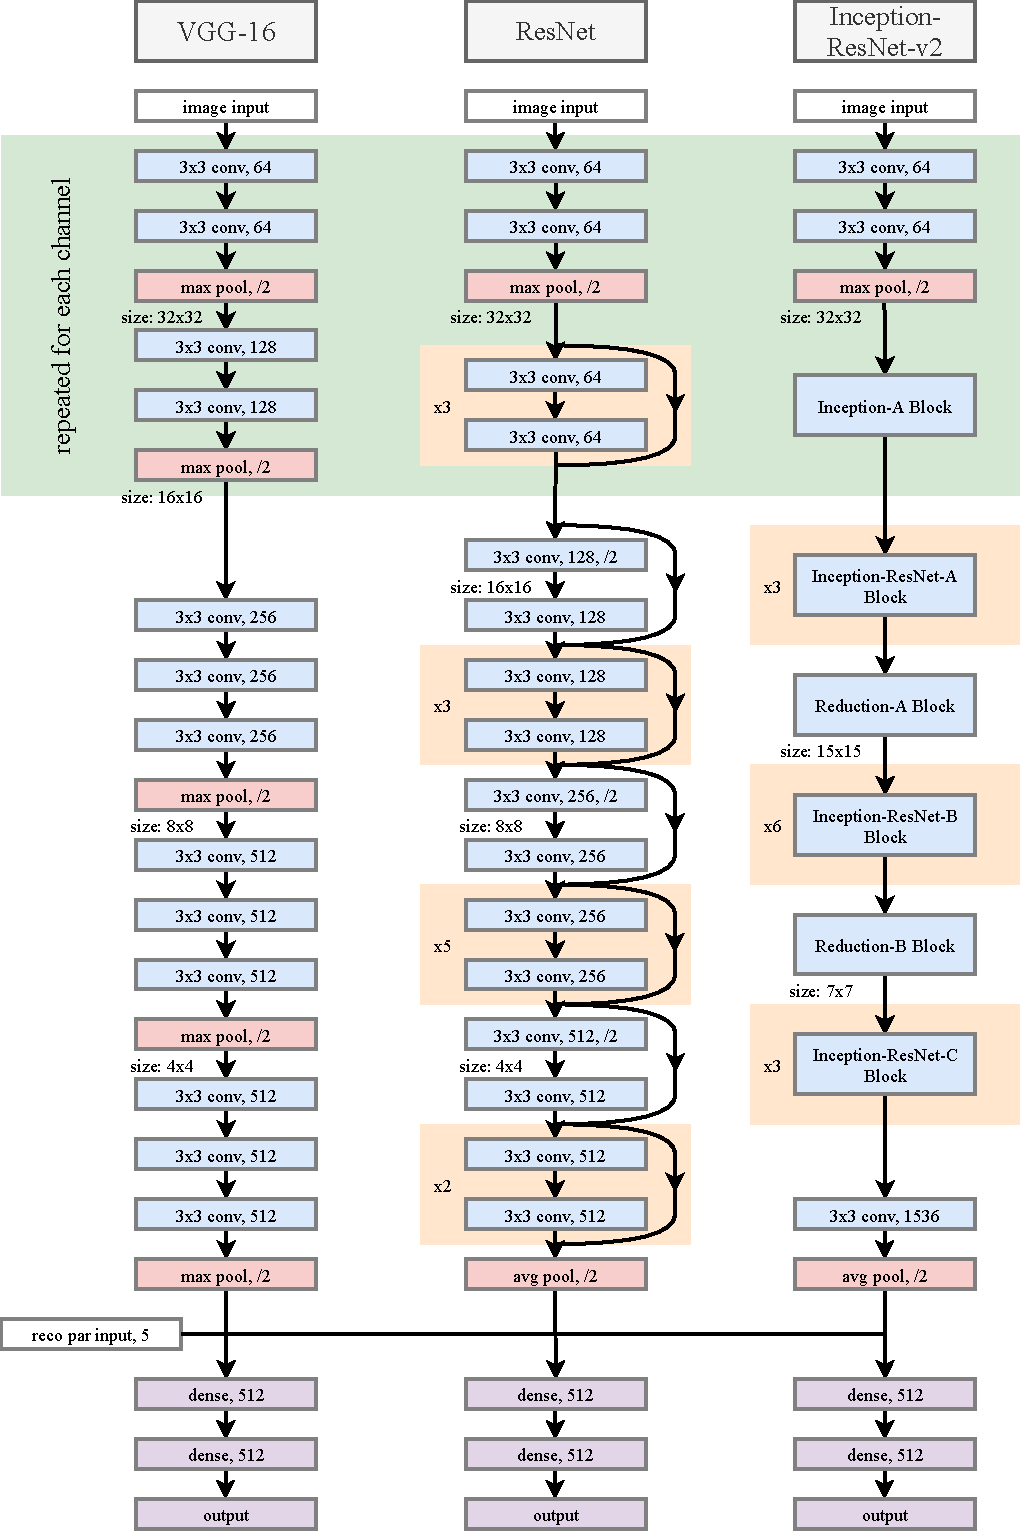
\includegraphics[width=0.8\textwidth]{diagrams/6-cvn/chipsnet.pdf}
    \caption[chipsnet short]
    {chipsnet long}
    \label{fig:chipsnet}
\end{figure}

\begin{figure}
    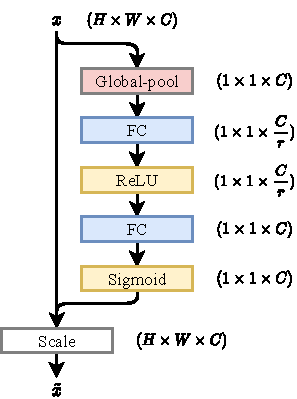
\includegraphics[width=0.8\textwidth]{diagrams/6-cvn/se.pdf}
    \caption[se short]
    {se long}
    \label{fig:se}
\end{figure}

\begin{figure}
    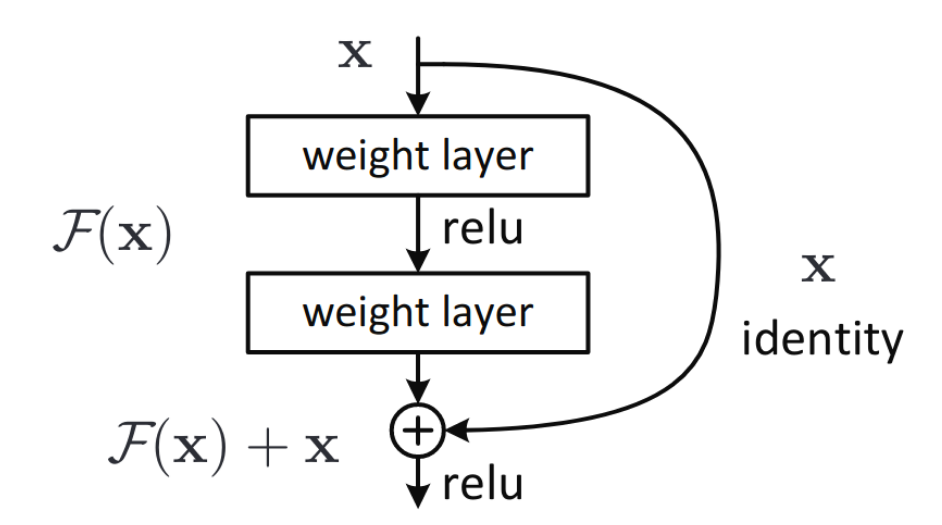
\includegraphics[width=0.8\textwidth]{diagrams/6-cvn/resnet_unit.png}
    \caption[resnet unit short]
    {resnet unit long}
    \label{fig:resnet_unit}
\end{figure}

\begin{figure}
    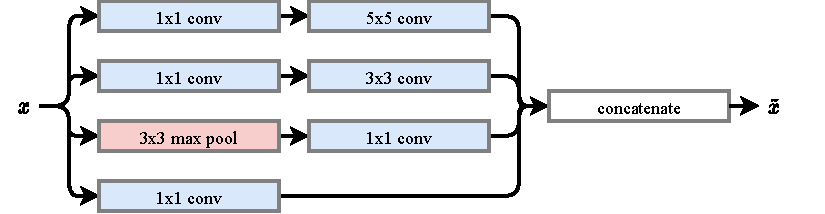
\includegraphics[width=0.8\textwidth]{diagrams/6-cvn/inception.pdf}
    \caption[inception short]
    {inception long}
    \label{fig:se}
\end{figure}

TODO: Get the detailed descriptions for the example events to put in the captions
\begin{figure}
    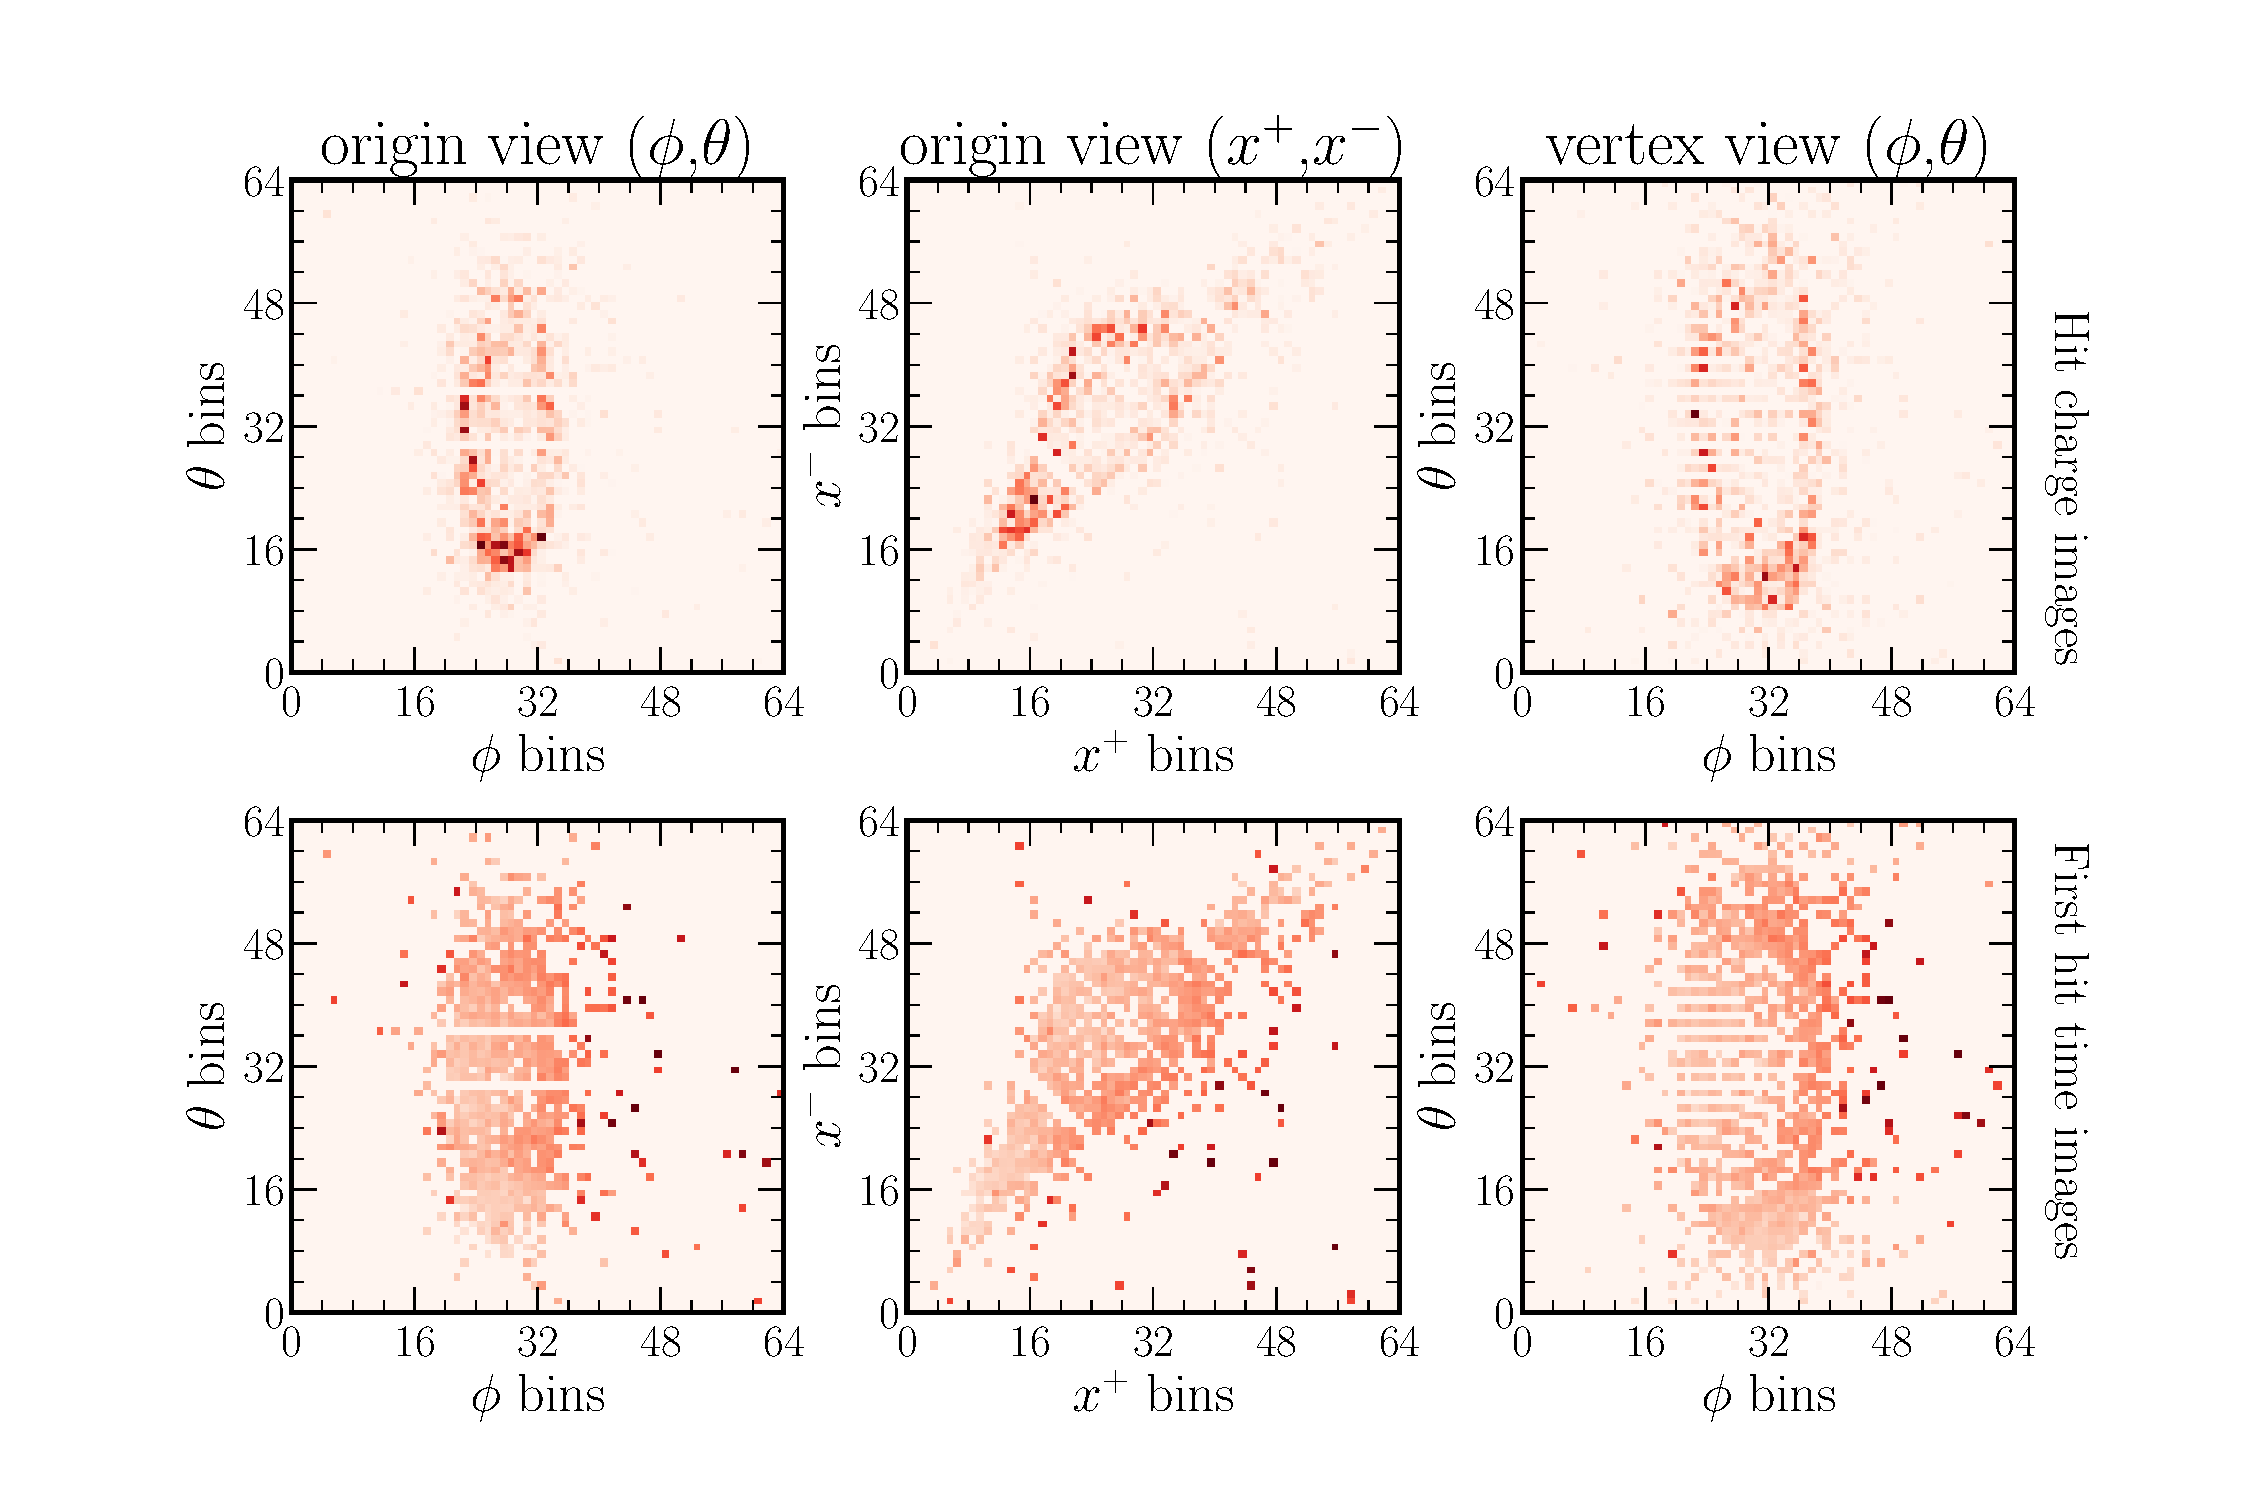
\includegraphics[width=\textwidth]{diagrams/6-cvn/chipsnet/explore_nuel_ccqel_event.pdf}
    \caption[explore nuel ccqel event short]
    {explore nuel ccqel event long}
    \label{fig:explore_nuel_ccqel_event}
\end{figure}

\begin{figure}
    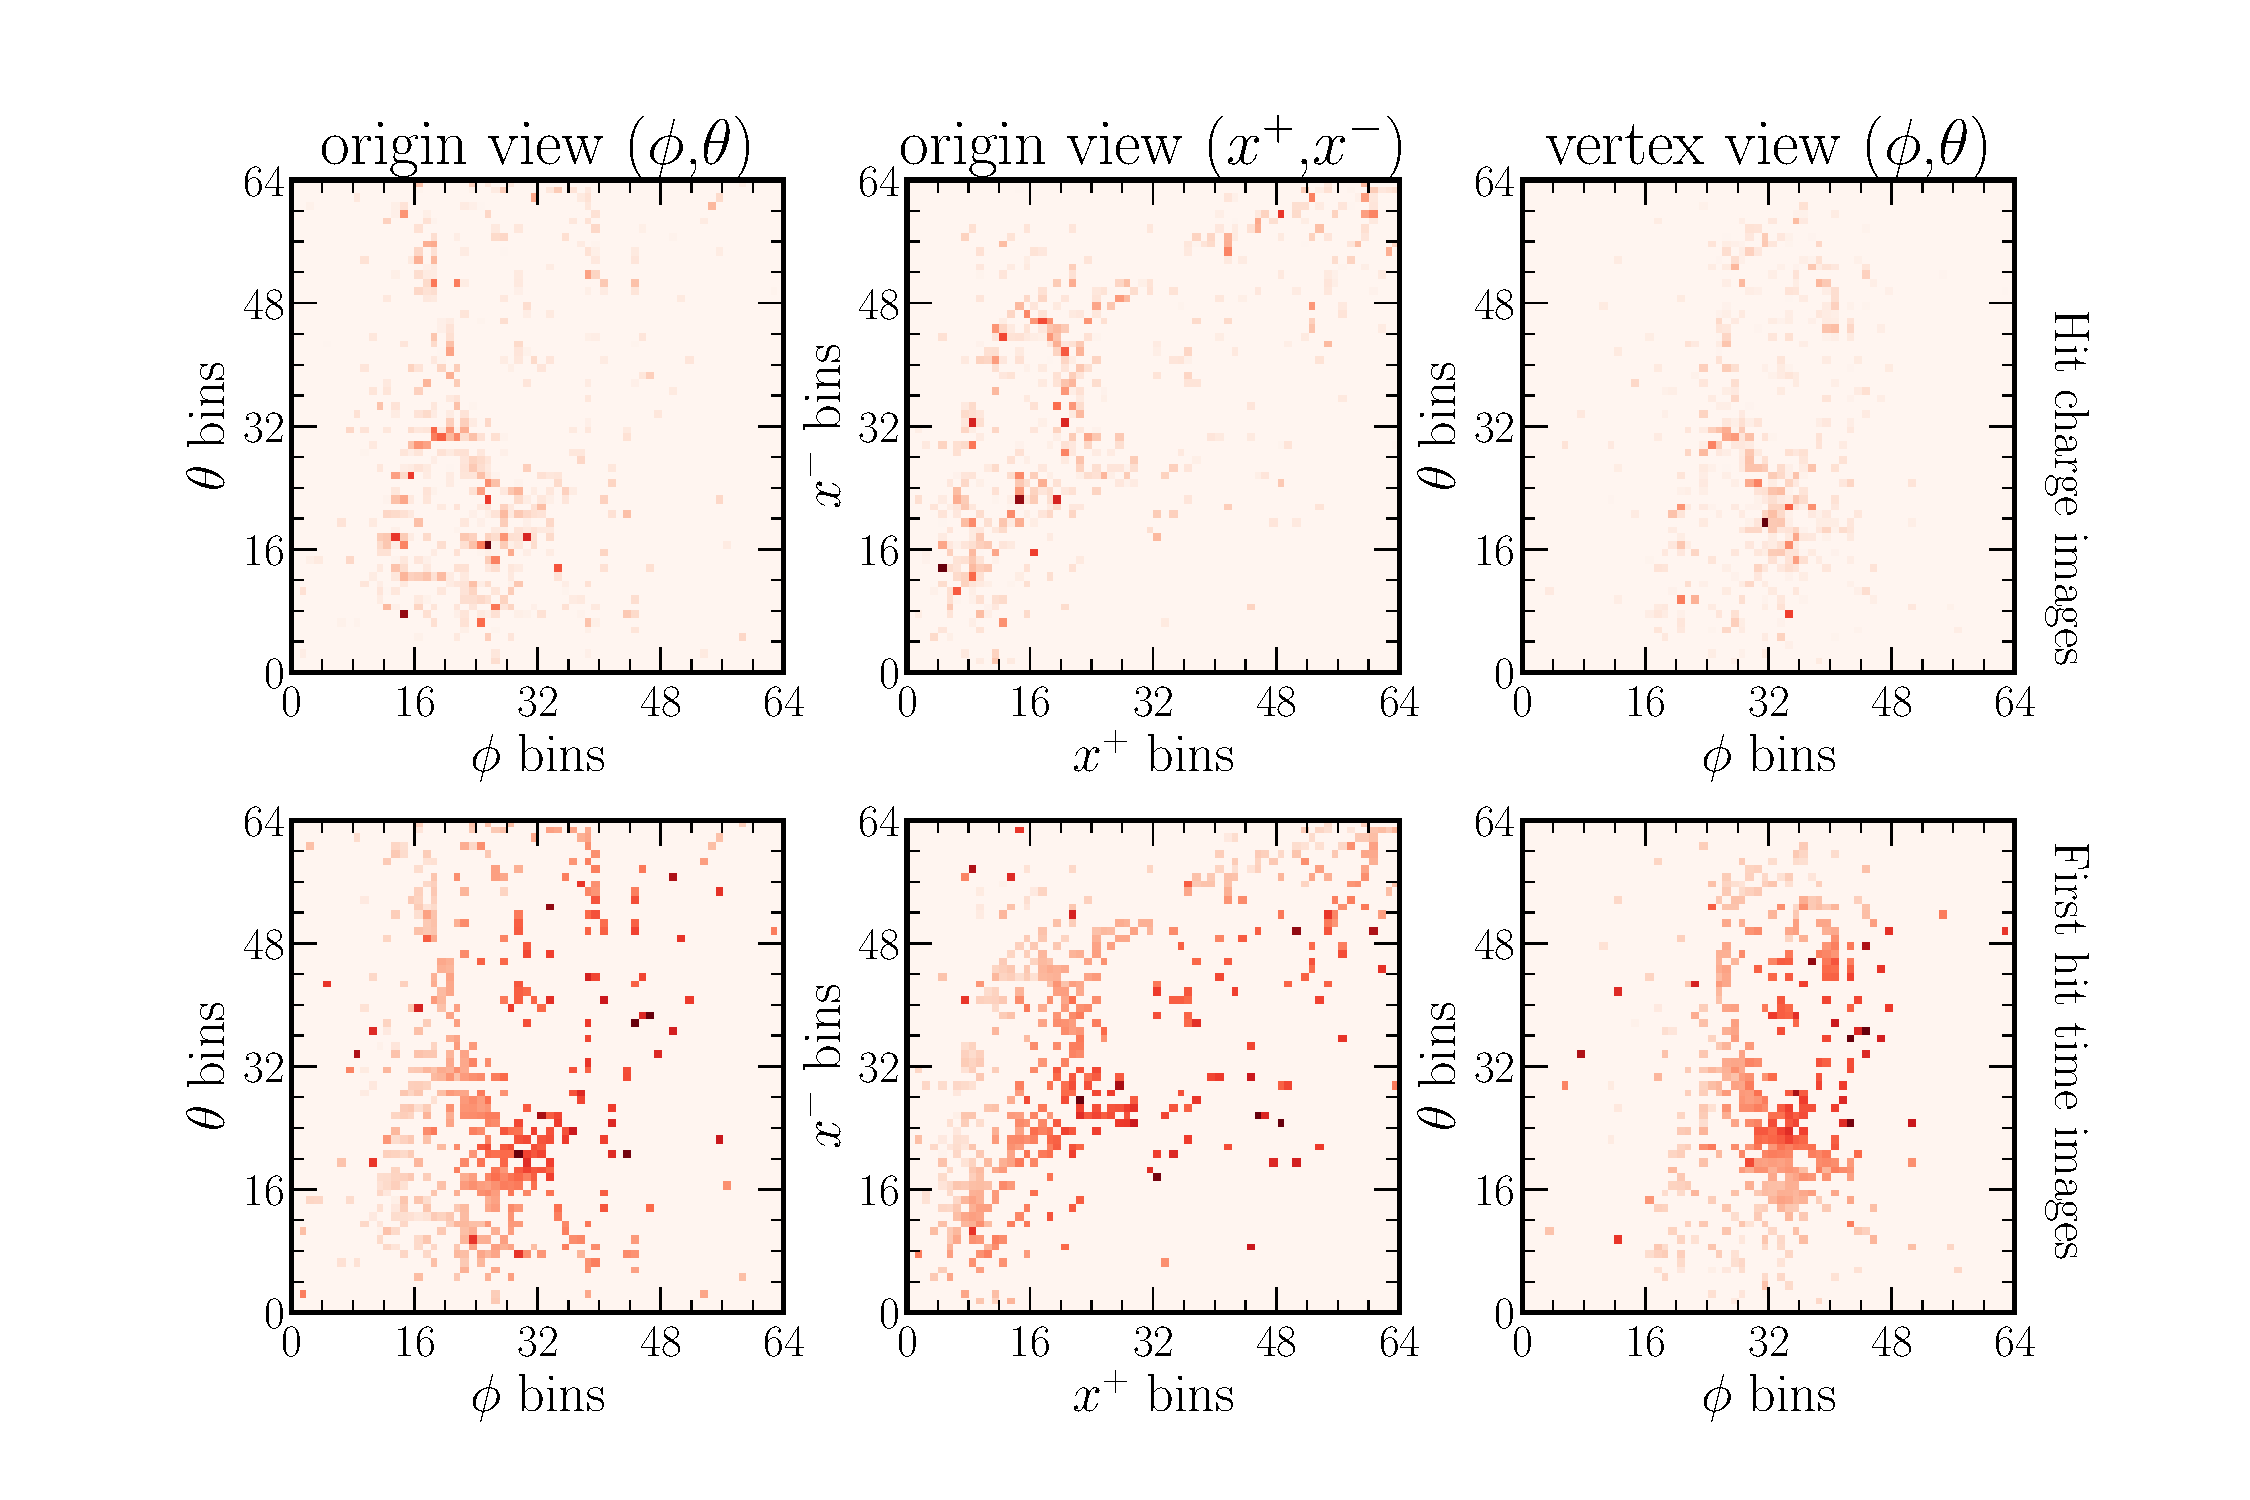
\includegraphics[width=\textwidth]{diagrams/6-cvn/chipsnet/explore_numu_ccdis_event.pdf}
    \caption[explore numu ccdis event short]
    {explore numu ccdis event long}
    \label{fig:explore_numu_ccdis_event}
\end{figure}

\begin{figure}
    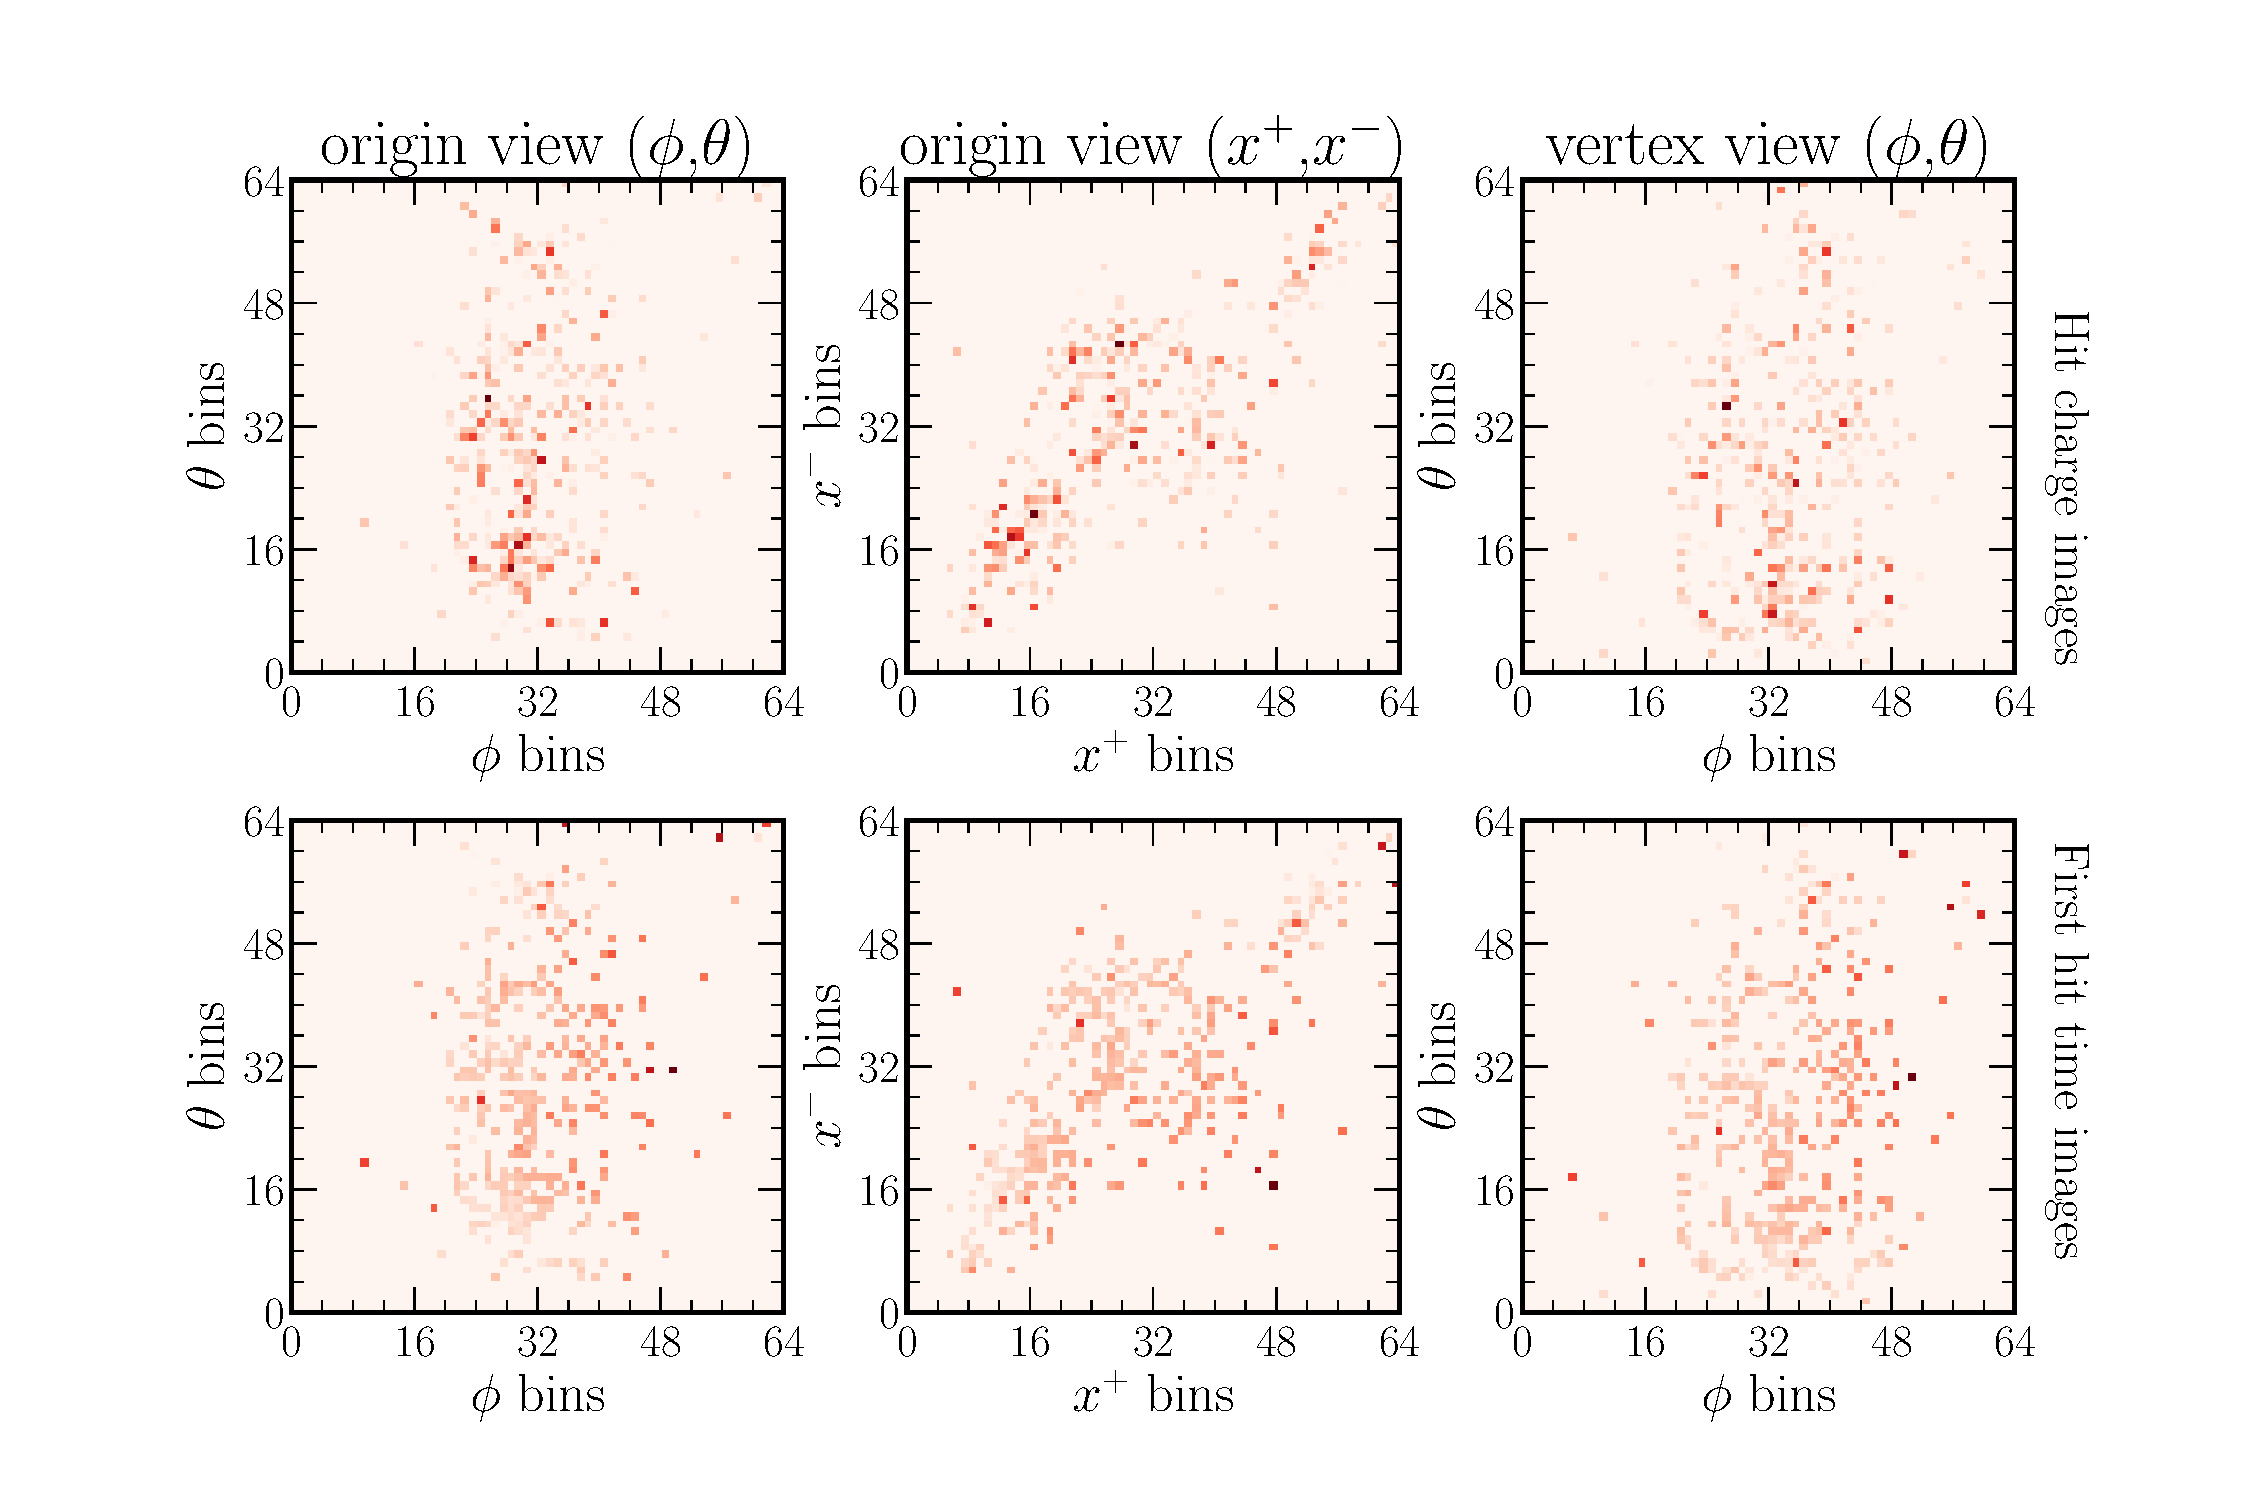
\includegraphics[width=\textwidth]{diagrams/6-cvn/chipsnet/explore_numu_ncdis_event.pdf}
    \caption[explore numu ncdis event short]
    {explore numu ncdis event long}
    \label{fig:explore_numu_ncdis_event}
\end{figure}

\begin{figure}
    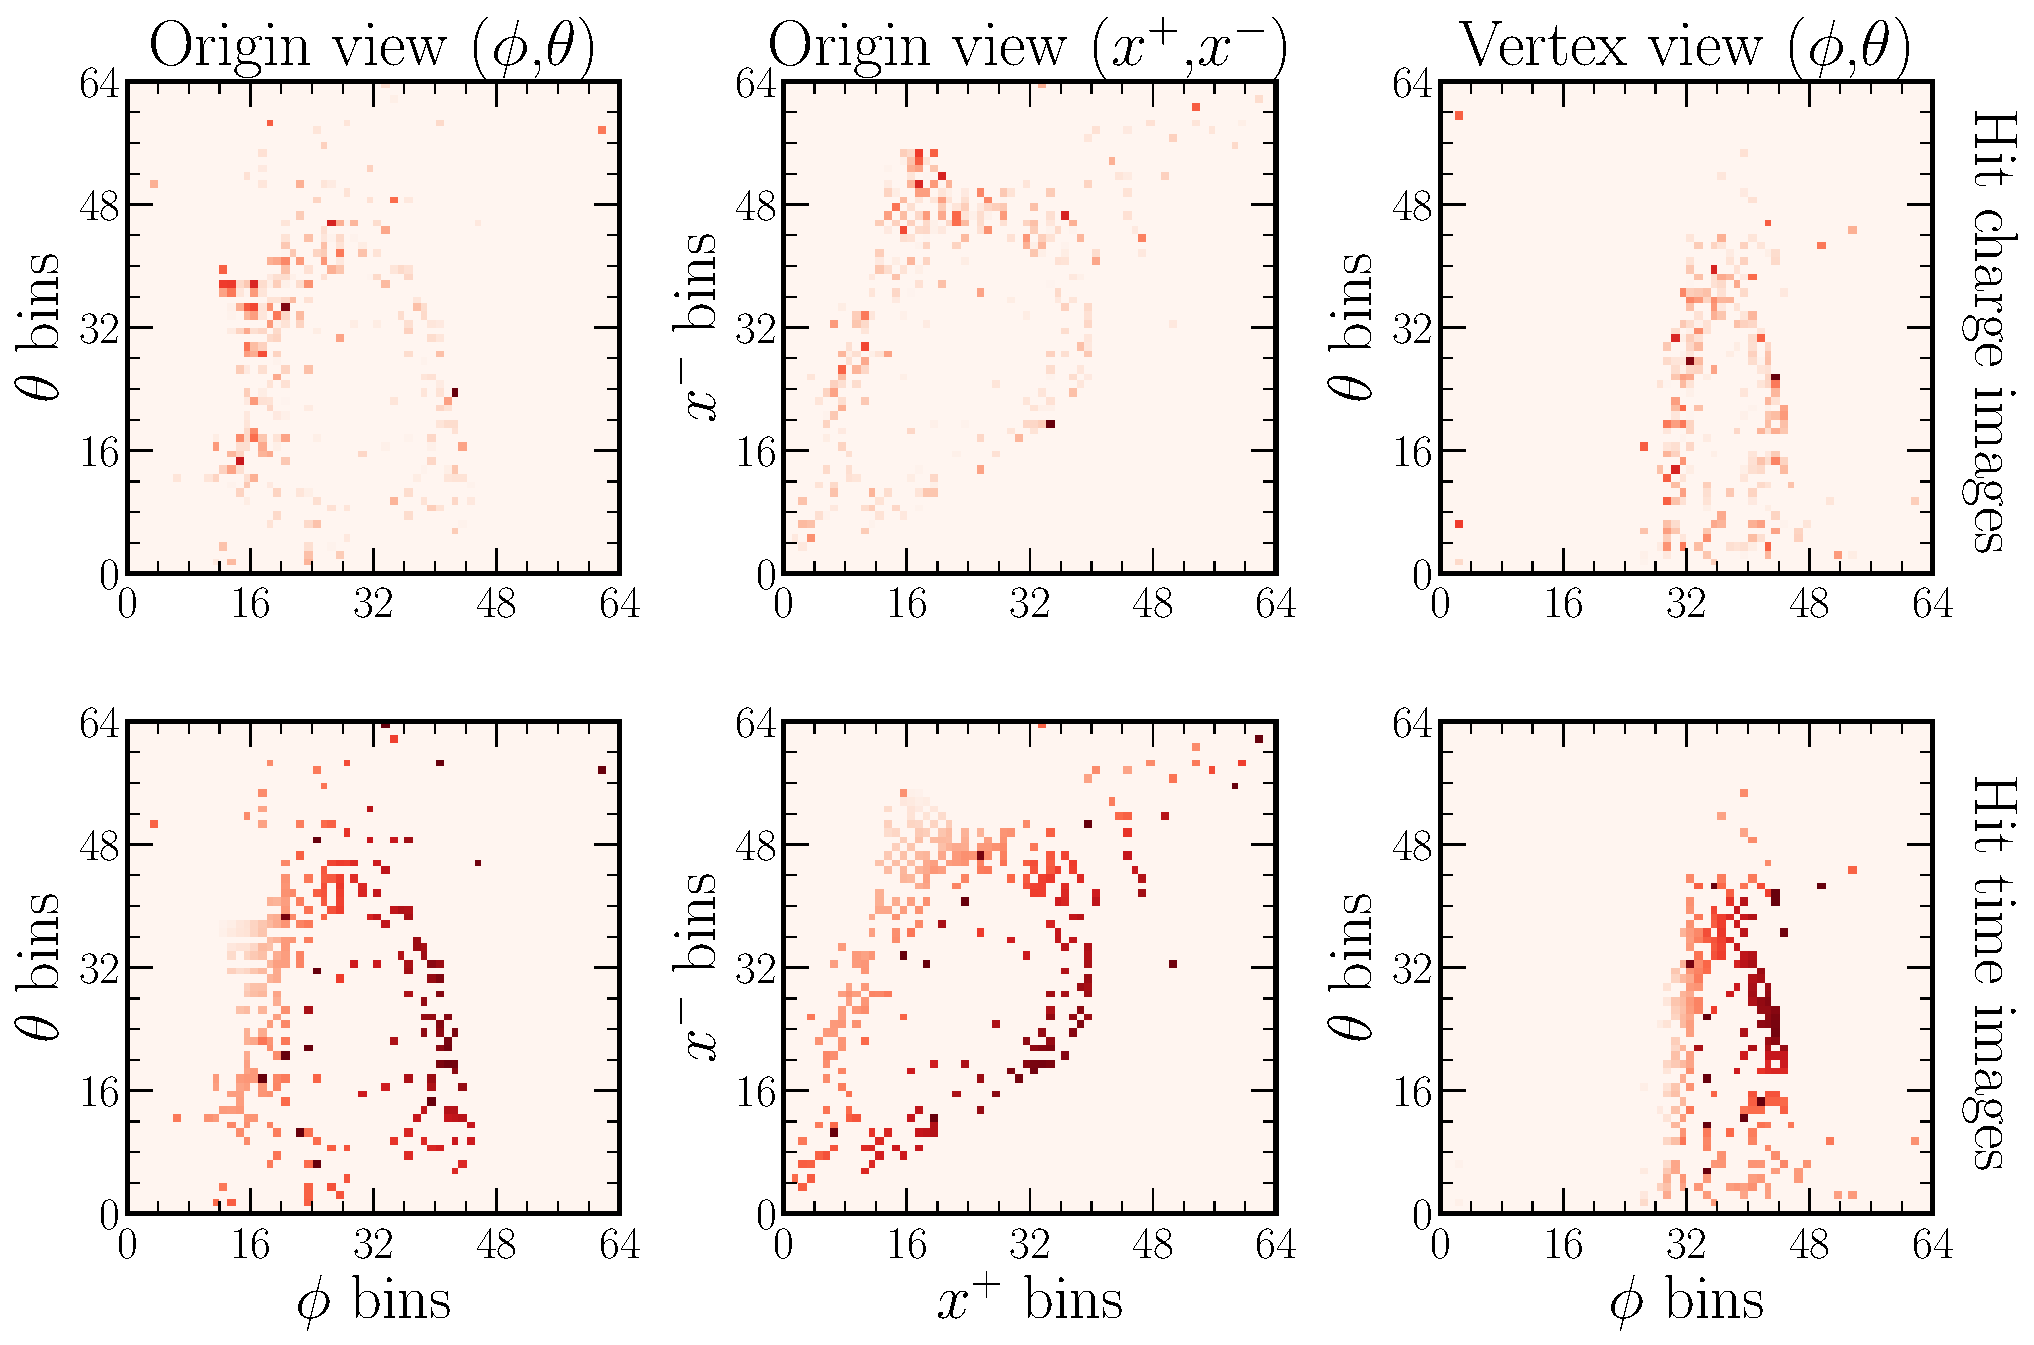
\includegraphics[width=\textwidth]{diagrams/6-cvn/chipsnet/explore_cosmic_event.pdf}
    \caption[explore cosmic event short]
    {explore cosmic event long}
    \label{fig:explore_cosmic_event}
\end{figure}

\begin{figure}
    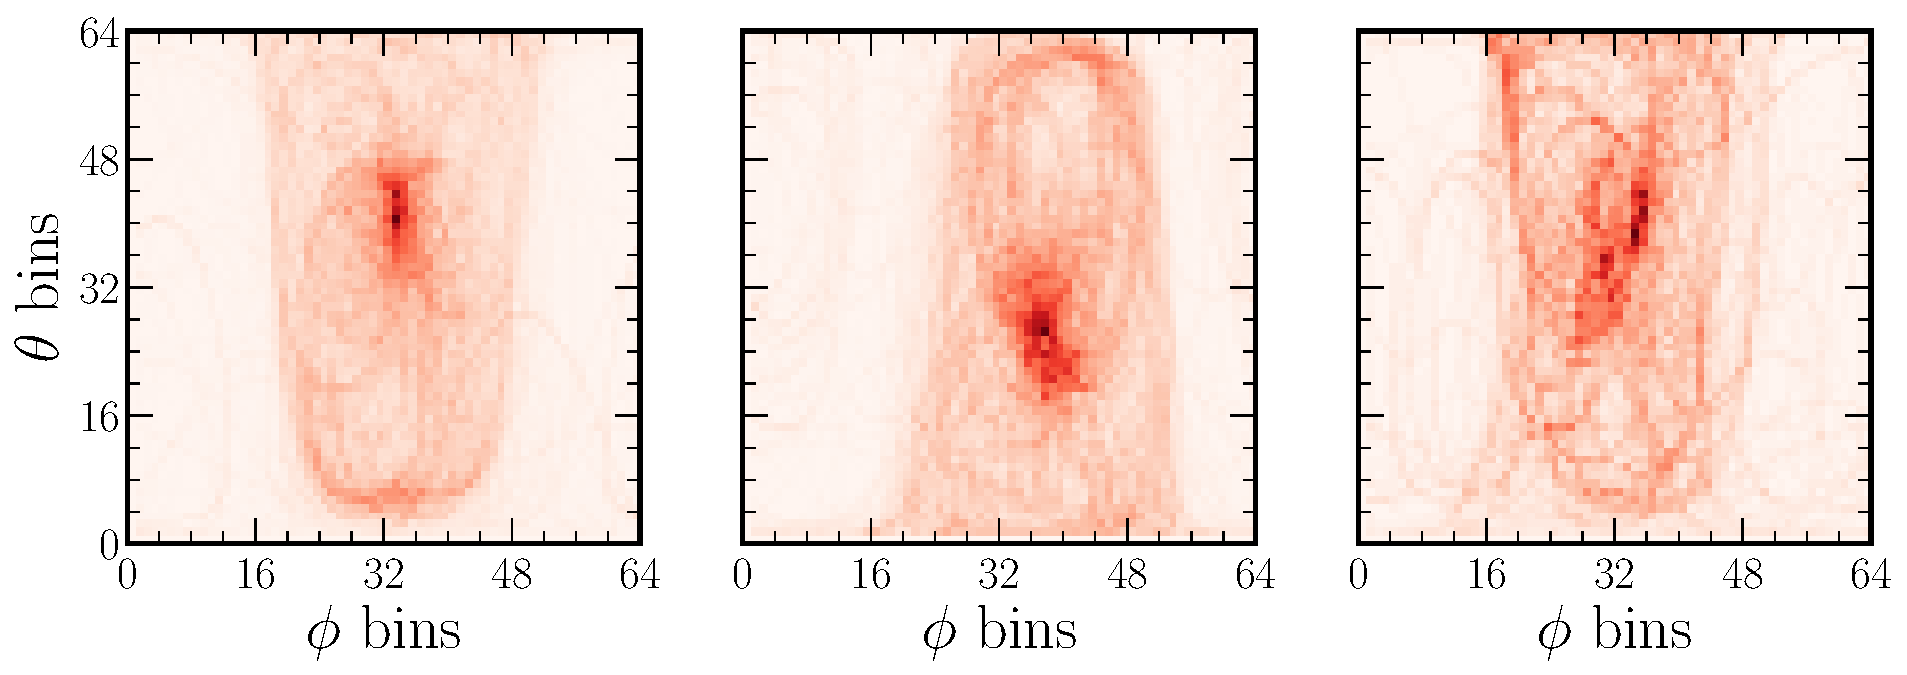
\includegraphics[width=\textwidth]{diagrams/6-cvn/chipsnet/explore_hough_events.pdf}
    \caption[example hough events short]
    {example hough events long}
    \label{fig:example_hough_events}
\end{figure}

\begin{figure}
    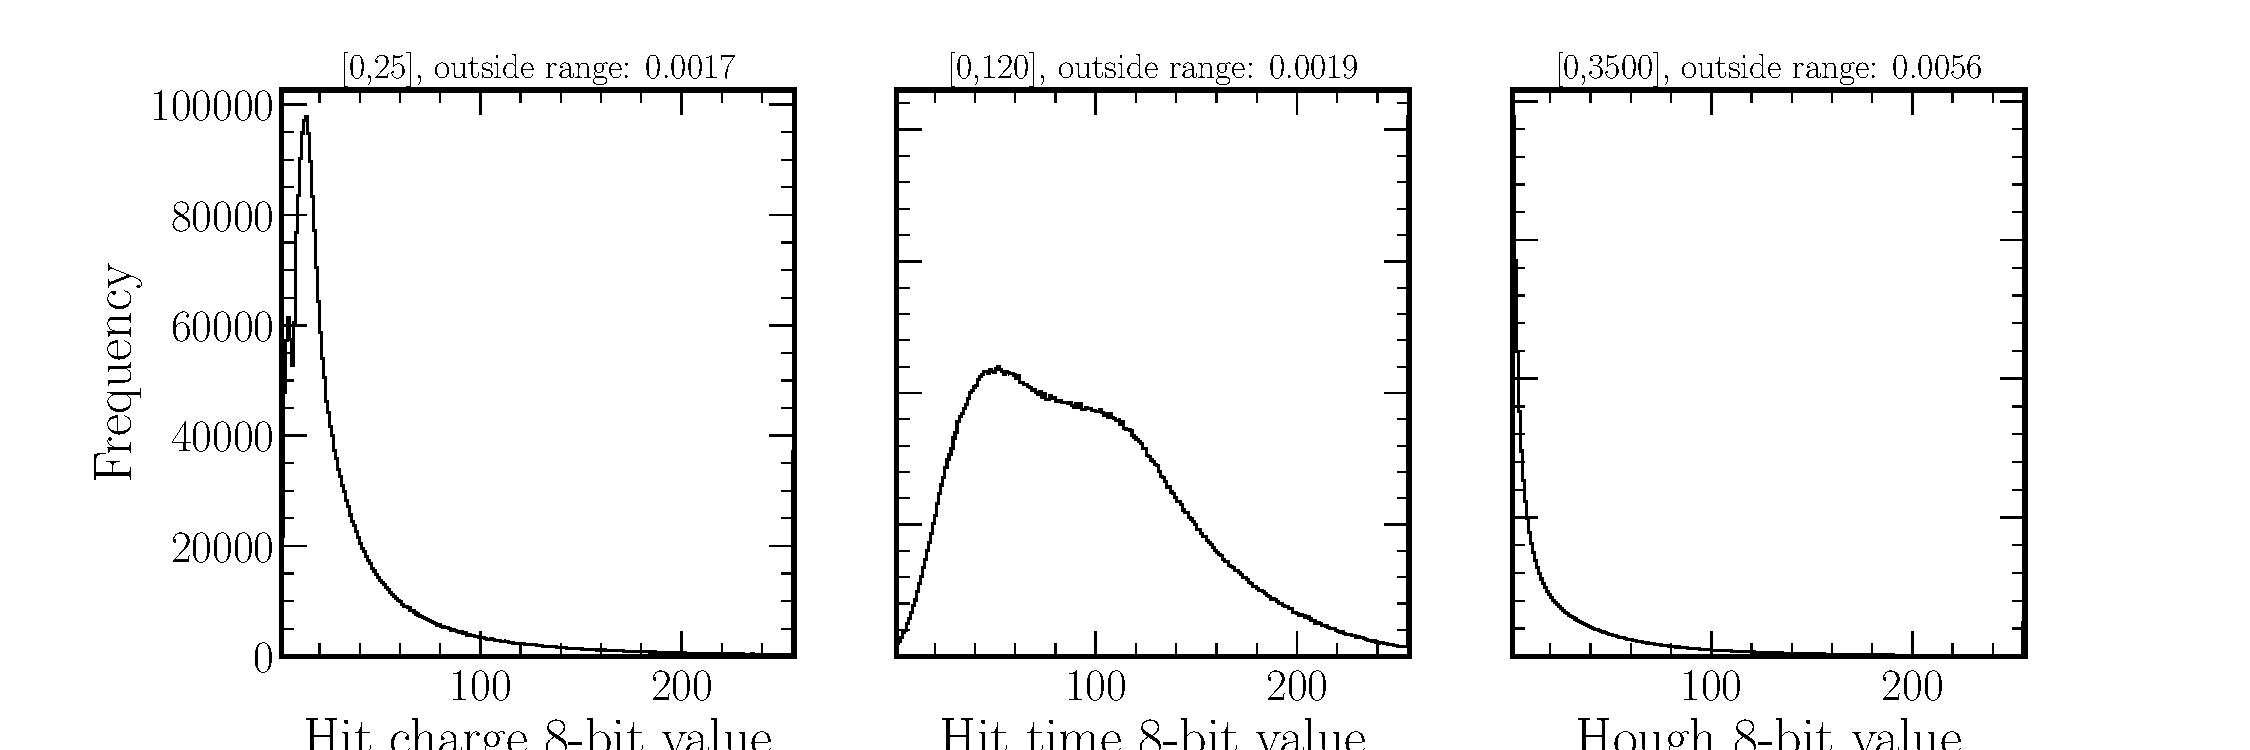
\includegraphics[width=\textwidth]{diagrams/6-cvn/chipsnet/expore_8_bit_range.pdf}
    \caption[explore 8 bit range short]
    {explore 8 bit range long}
    \label{fig:explore_8_bit_range}
\end{figure}

\begin{figure}
    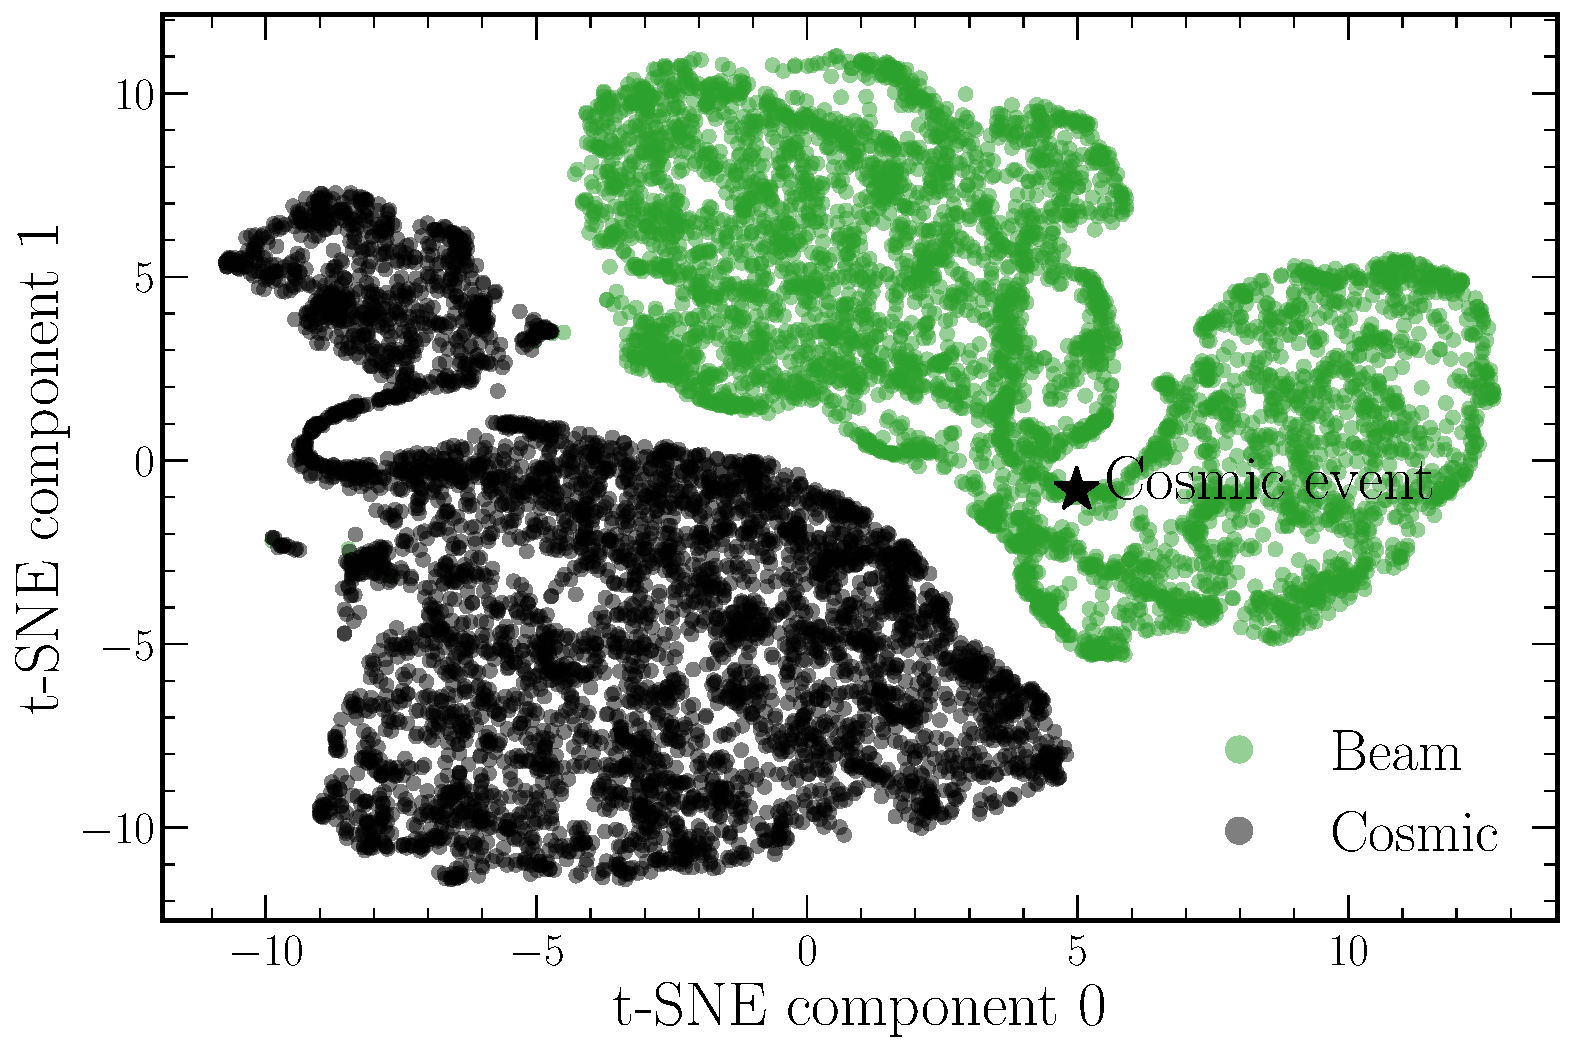
\includegraphics[width=\textwidth]{diagrams/6-cvn/chipsnet/final_cosmic_tsne.pdf}
    \caption[final cosmic tsne short]
    {final cosmic tsne long}
    \label{fig:final_cosmic_tsne}
\end{figure}

\begin{figure}
    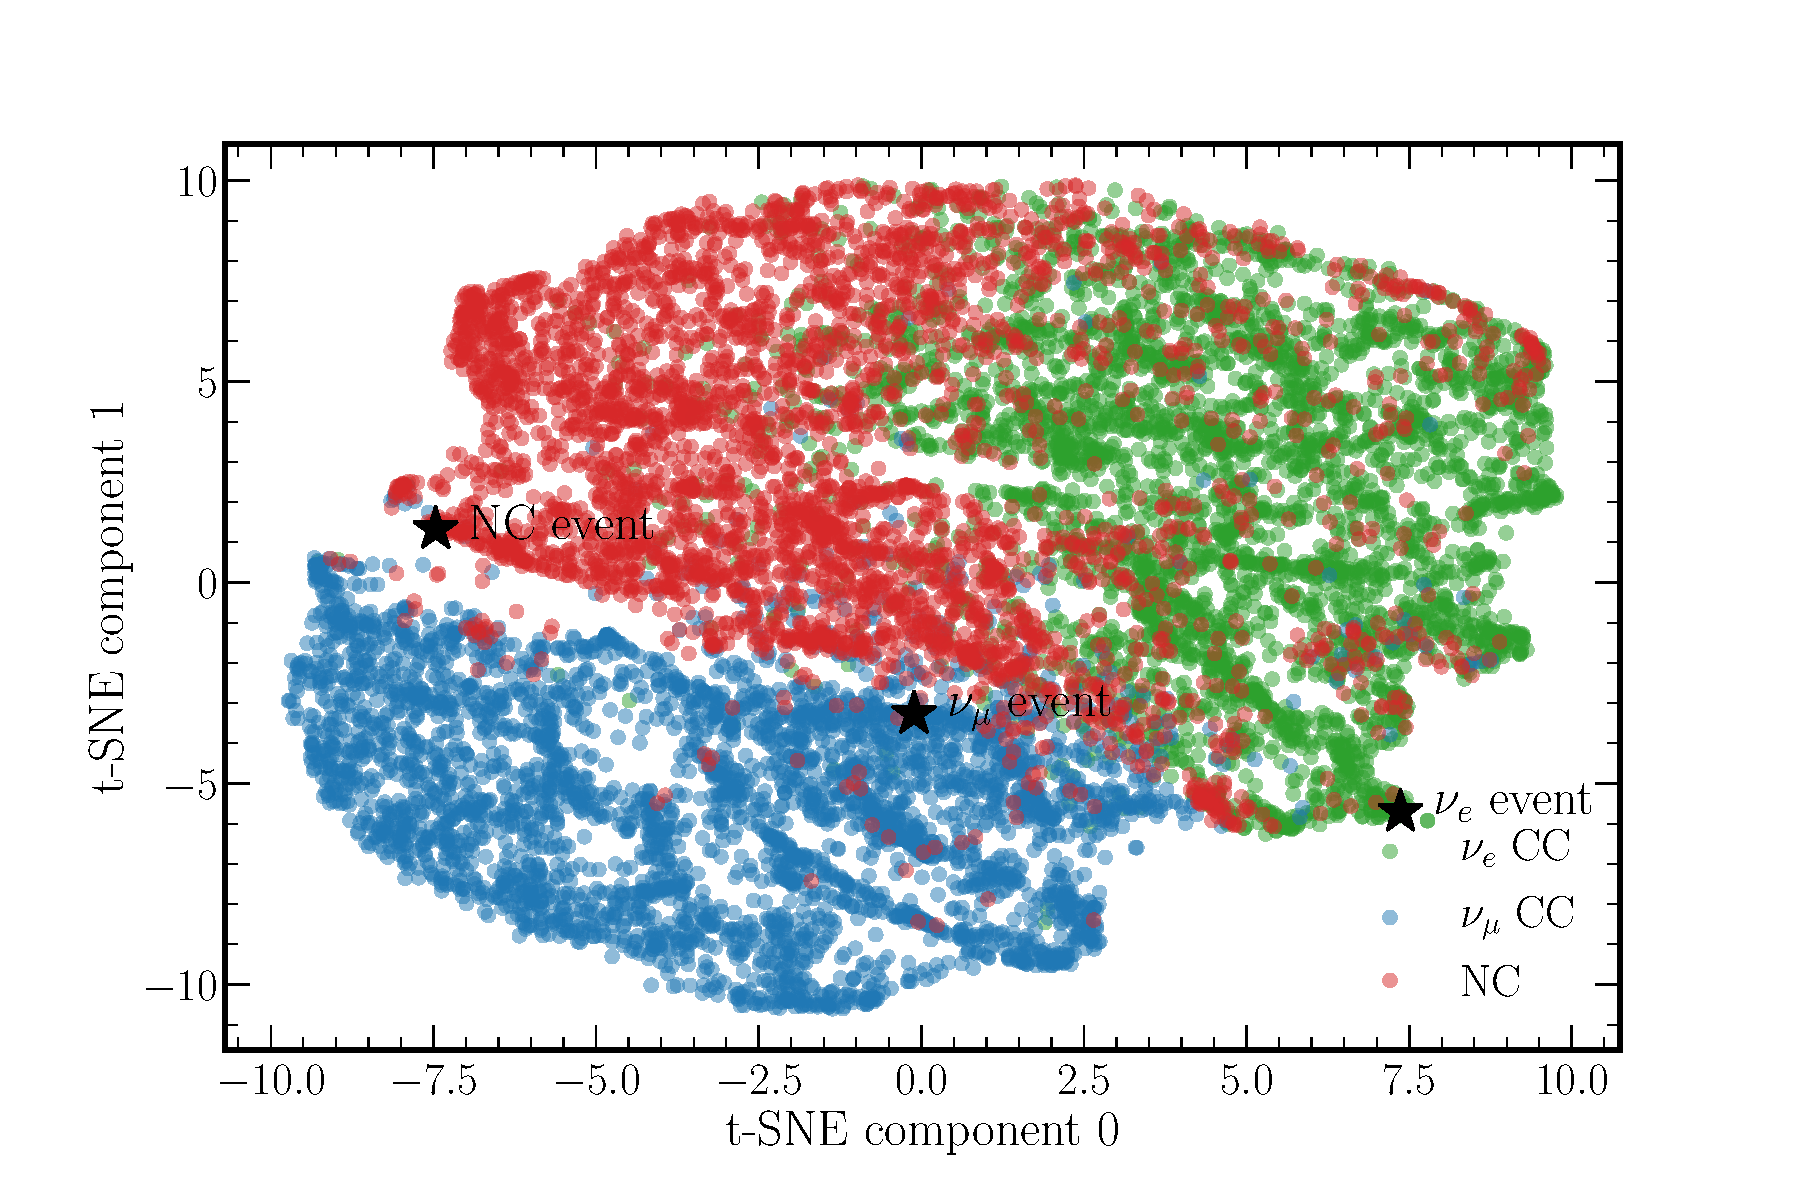
\includegraphics[width=\textwidth]{diagrams/6-cvn/chipsnet/final_beam_tsne.pdf}
    \caption[final beam tsne short]
    {final beam tsne long}
    \label{fig:final_beam_tsne}
\end{figure}

\begin{figure}
    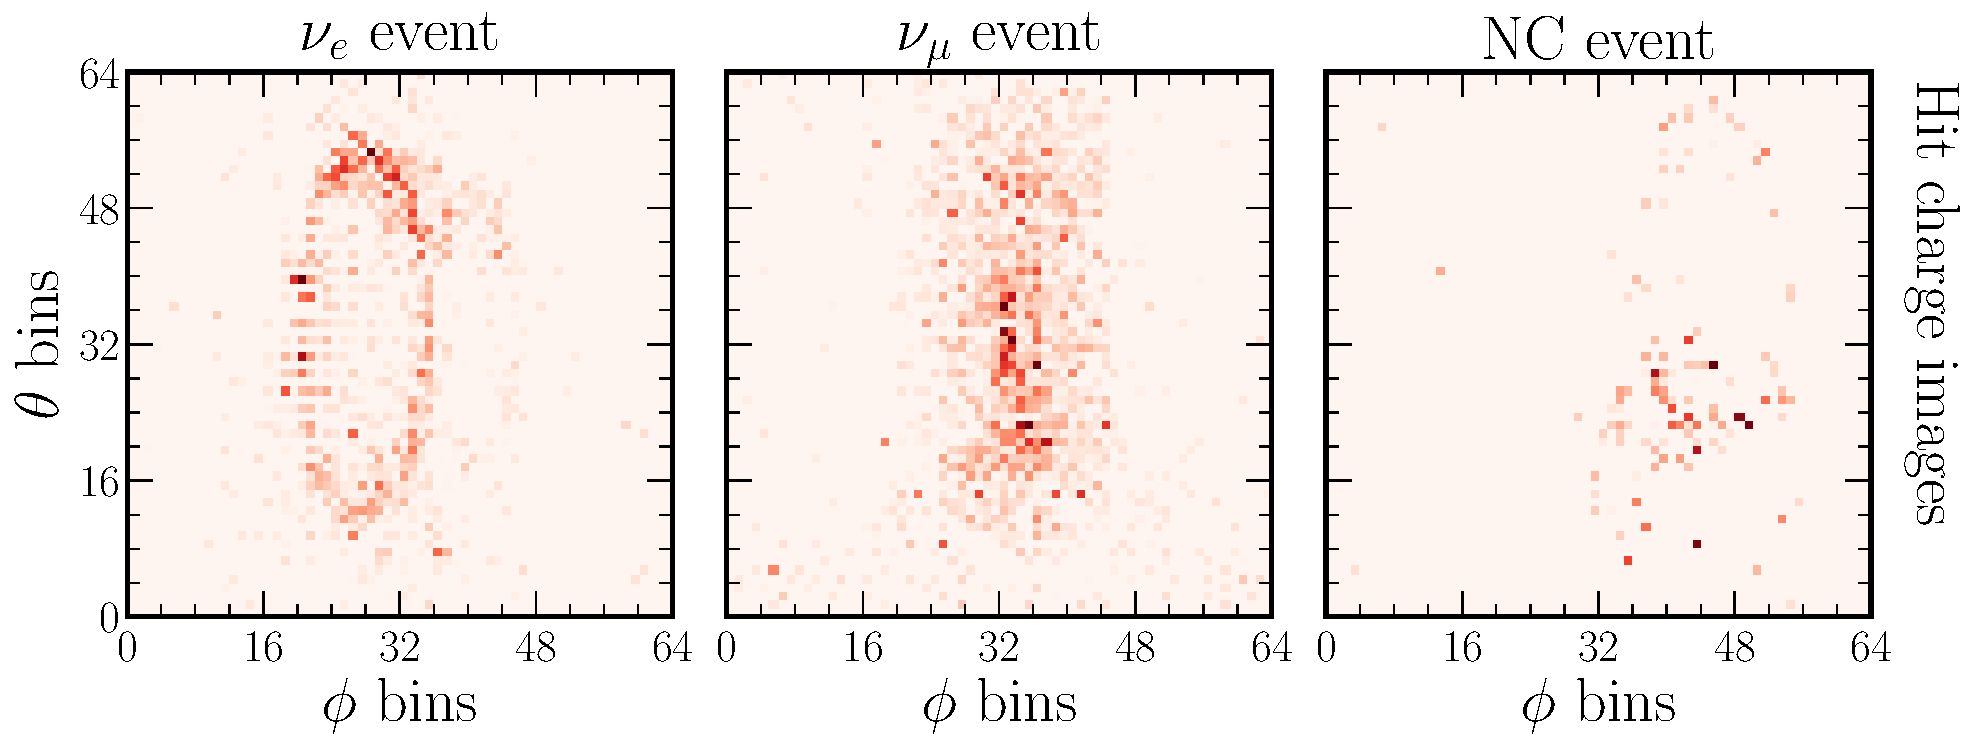
\includegraphics[width=\textwidth]{diagrams/6-cvn/chipsnet/final_beam_tsne_events.pdf}
    \caption[final beam tsne events short]
    {final beam tsne events long}
    \label{fig:final_beam_tsne_events}
\end{figure}

DIAGRAM: True neutrino energy distributions for different categories for energy estimation.
DIAGRAM: Neutrino energy and estimated neutrino energy distributions on same plots.
INFO: Table of the final number of expected events and efficiency and purity of the signal at the chosen cut value (nuel and numu)
DIAGRAM: Parrallel coordinates plots for tuning the hyperparameters
INFO: Time taken comparison with old reconstruction (just inference time for all stages)
DIAGRAM: Final stacked reconstructed energy distribution of selected events given a number of years running
INFO: Super-k/Dune/Nova comparison numbers for effeciencies and energy resolutions etc...
DIAGRAM: Table of how succesive cuts affect the selection of different event types
DIAGRAM: CP-Violation sensitivity from GLoBES with the new fluxes, efficiencies, smearing matrices etc... get from Tom/John

- In the future we could do semantic segmentation or use GANS

\section{References}

Cern summer report in Ref.~\cite{theodore2016}
CHIPS cosmic rate in Ref.~\cite{son2013}
Nova first CVN paper in Ref.~\cite{aurisano2016}
- CNN's have been widely applied in various computer vision tasks to solve image recongnition and analysis problems.
- The core problem in HEP is the correct categorisation of particle interactions
- This is usually done by reconstructing high-level componenets suh as clusters, tracks, showers, jets and rings. and
then summarising these objects energies, directions and shapes, these wuantities are then fed into k-nearest neighbours,
BDTs or MLPs to seperate sign from bkg.
- Prone to failure, mistakes in the reconstruction, and limitation to what has been implemented by humans.
- computer vision moved away from specifically constructed features to sing ML CNNs to discover the features.
- Manu HEP problems including water cherenkov detectors essentially result in an 'image' of an event, which are well suited to these tools.
- MLP are widely used in HEP,
Nova context enriched CVN paper in Ref.~\cite{psihas2019}
Nova energy recontruction CVN in Ref.~\cite{baldi2019}
MicroBooNE CNN paper in Ref.~\cite{acciarri2017}
Watchmal/Triumf Cherenkov variational autoencoders in Ref.~\cite{abhishek2019}
Daya bay paper in Ref.~\cite{racah2016}
SHiP GAN simulation paper in Ref.~\cite{ahdida2019}
New ideas with x+ x- mapping in Ref.~\cite{berns2020}
DUNE TDR in Ref.~\cite{abi2020}
DUNE CVN paper in Ref.~\cite{collaboration2020}
Initial CNN visualisation paper in Ref.~\cite{zeiler2013}
Original t-SNE paper in Ref.~\cite{maaten2008}
Original 'dropout' paper in Ref.~\cite{hinton2012}
Original Batch normalisation paper in Ref.~\cite{ioffe2015}
VGG paper in Ref.~\cite{simonyan2014}
Improved resnet paper in Ref.~\cite{he2016}
Inception-resnet paper in Ref.~\cite{szegedy2016}
Squeeze-and-excitation networks paper in Ref.~\cite{hu2017}
MobileNetV2 paper in Ref.~\cite{sandler2018}
EfficientNet paper in Ref.~\cite{tan2019}
Multi-task learning how to weight paper in Ref.~\cite{kendall2017}
Bag of tricks in Ref.~\cite{he2018}
Grad-CAM paper in Ref.~\cite{elvaraju2019}
Amazing machine learning for physicists thing in Ref.~\cite{mehta2019}
- Deep neural networks have emerged as one of the most powerful supervised learning techniques.
- They truly caught the attention of the wider ML communityr in 2012 when A. Krizhevsky, I, Sutskever and G. Hinton used a GPU to train
AlexNet, lowering the error rate on the image classification task ImageNet by 12%. 
- Such was the rapid pace of advance afterwards that the ResNet model acheived a 3.57\percent error just three years later.
- Many high level libraries have now been formed, predominently led by Tensorflow (from google) and pyTorch (from facebook) making it easier to quickly code and implemenetd DNNs.
- Neural networks are neural-inspired nonlinear models for supervised learning. Constructed from the basic building blocks of a "neuron".